% !TEX root = ../main.tex
\clearpage
\section{应用价值与发展方向}
\subsection*{应用价值与发展方向}\label{page:48}
\ifdraftversion{\noindent\small\color{gray}写作页位 48\quad 负责人 武桐宇\par}\fi

\textbf{本页结论：}本项目的近期价值是让低空研究讨论能回到来源、关系与规则；其长期价值取决于是否持续补齐真实授权数据、核验图谱关系并形成可审计的协作机制。

\begin{table}[htbp]
\centering
\caption{应用价值、受益对象与成立条件}
\label{tab:wty-application-value}
\small
\begin{tabularx}{\linewidth}{p{0.22\linewidth}X p{0.24\linewidth}}
\toprule
价值方向 & 可能受益对象 & 成立条件 \\
\midrule
研究可复核性 & 课程、研究小组、产业研究人员 & 事件原文、版本和公式均可定位 \\
跨学科协作 & 产业、技术与财务背景不同的协作者 & 术语、状态和关系边界被共同维护 \\
数据治理训练 & 数据维护与产品运营人员 & 来源、权限、清洗和撤回流程落地 \\
后续工具扩展 & 有授权数据和明确业务场景的团队 & 通过安全、许可和人工复核后再接入 \\
\bottomrule
\end{tabularx}
\end{table}

\begin{figure}[htbp]
\centering
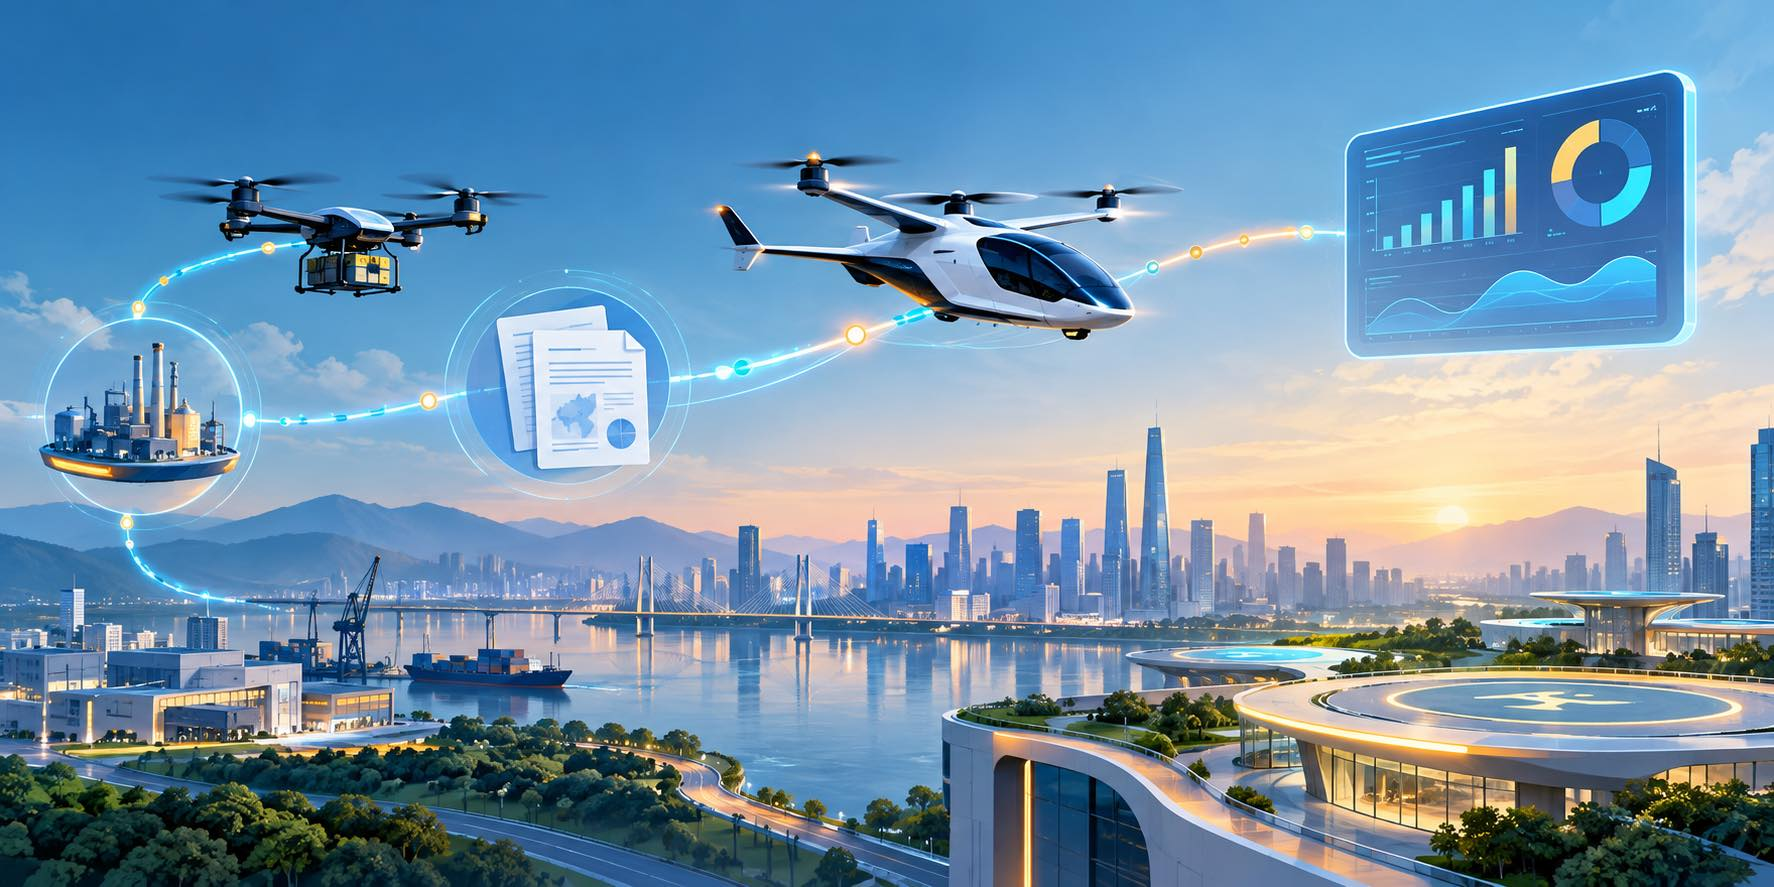
\includegraphics[width=0.88\linewidth]{assets/Eazin-stefan3199/low-altitude-research-ecosystem.jpg}
\caption{低空研究生态的概念示意图（AI生成概念图，不表示真实部署、客户或运营结果）}
\label{fig:wty-research-ecosystem}
\end{figure}

下一步不应以增加概念标签为目标，而应优先完成来源失效复查、待核验关系补证、真实数据授权评估和小范围任务验证。只有当这些前提满足后，才讨论更广泛的产品化或商业化。
